\documentclass[a4paper,10pt]{article}

\usepackage[dvipsnames]{xcolor}
\usepackage[margin=1in]{geometry}
\usepackage{amsmath}
\usepackage{graphicx}

\title{Quiz 1 }
\author {Victoria Deng} 
\date{\small August 2020}
\begin{document}
\maketitle

\section*{Lecture 2 - Perspective and Polygonal Geometry}
\textcolor{SeaGreen}{\textbf{Pinhole Camera Model:}} A simple setup where there is a hole on one side that projects an image. In reality would be reflected upside down, however for the purposes of computer graphics, we project the image in front of the object. 
\\ \\
\textcolor{SeaGreen}{\textbf{Modelling a Virtual Camera:}} \\ 
\begin{figure}[htbp]
\centerline{ 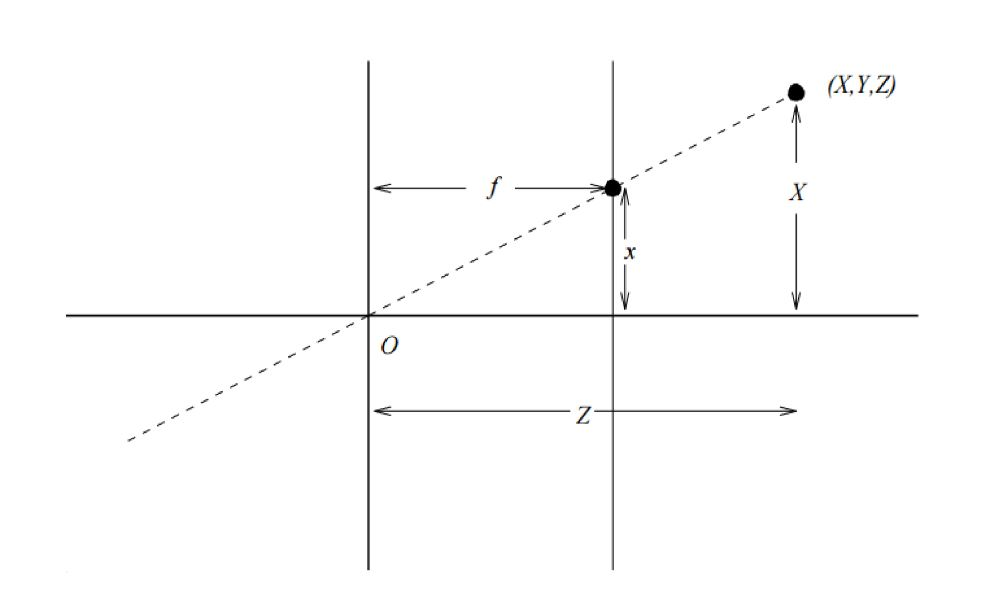
\includegraphics[scale = 0.5]{projimage}}
\caption{Perspective diagram of virtual camera geography, X is the object being projected }
\label{fig}
\end{figure}

\noindent \textcolor{SeaGreen}{\textbf{Perspective Formulas:}}  Applicable only for camera-centred coordinates. \\ 
\begin{center} 
$\frac{x}{f} = \frac{X}{Z} $ \\ 
$\frac{y}{f} = \frac{Y}{Z} $ \\ 
\end{center}

\noindent \textcolor{SeaGreen}{\textbf{Virtual Camera Geometry:}} The image project surface is imagined to be in front of a projection centre, the projected image would be geometrically equivalent to the object's dimensions. \\ \\
\noindent \textcolor{SeaGreen}{\textbf{Perspective Projection:}} Requires width, height and length to draw a 3D image. Depth is also conveyed depending on the number of point-perspectives required.\\ \\
\noindent \textcolor{SeaGreen}{\textbf{Horizon line:}} Key component of perspective modelling, the horizon line is considered eye level. \\ \\
\noindent \textcolor{SeaGreen}{\textbf{Vanishing Points:}} Point in linear perspective, the point where all vanishing lines should converge. Generally placed on the horizon line for 1 and 2 point perspectives.\\ \\
\noindent \textcolor{SeaGreen}{\textbf{Vanishing Lines:}} Lines that meet at the vanishing point on the horizon line. \\ \\
\noindent \textcolor{SeaGreen}{\textbf{X Point Perspective:}} The number of vanishing points in a model. Three point perspective has the vanishing point below the horizon line \\ \\ 
\newpage
\noindent \textcolor{SeaGreen}{\textbf{Polygon:}} Any plane figure bounded by straight line segements. Can be in the form of a polygonal arc (polylines or an open polygon), polygonal boundaries (a closed polygon) or filled polygons. \\  \\
\noindent \textcolor{SeaGreen}{\textbf{Representation of Polygons:}} Can be represented as a set of line segments (connected but unordered), or an ordered sequence of vertices using absolute or relative coordinates. The ordered sequence can allow for 'lazy rendering', as if part of a polygon is ont shown, then it doesn't need to be rendered. Another convention is walking order, where there is a sequence of vertices on the outside of a polygon and the inside of one. Generally the sequences are opposites, eg anti-clockwise for outside and clockwise for inner. \\ \\
\noindent \textcolor{SeaGreen}{\textbf{Polygon Types:}} Convex (All edges under 180 degrees), Concave (One edge above 180 degrees), Non-Simple (Two or more connected polygons), Star, Multiple Boundary (Hollow polygons inside a polygon).  \\ \\
\noindent \textcolor{SeaGreen}{\textbf{Level of Detail:}} Affected by the amount of polygons required to render an object. More polygons equals more details, however when using a model we need to balance the detail and the expense of rendering it. For instance, if we want to model a rabbit 100m away, is it necessary to use the most detailed model? \\ \\
\noindent \textcolor{SeaGreen}{\textbf{Summary:}} Polygons are used a lot for rendering, where the most common polygon used is a triangle as every other polygon is basically a bunch of triangles.  \\ 

\newpage
\section*{Lecture 3 - The Rendering Pipeline (Direct3D)}
\noindent \textcolor{ForestGreen}{\textbf{Pipeline Stages:}} Represented in the order that they are executed in the Direct3D pipeline  \\\\
\noindent \textcolor{ForestGreen}{\textbf{Input Assembler:}} Building block stage, main purpose is reading in the data from our buffers then transforming it into a primitive format to be used by the rest of the pipeline. Generally use triangle lists for defining triangles rather than individually defining vertices.\\\\
\noindent \textcolor{ForestGreen}{\textbf{Vertex Shader:}} Performs operations on indivual vertices from the Input Assember, typically involves transforming them or bringing them into the world/scene.  \\\\
\noindent \textcolor{ForestGreen}{\textbf{Tesselation Stages:}} Optional, but used to add details and smooth out triangles. Can take models with lower details and render in higher details, or generate additional vertices. \\\\
\indent \textcolor{ForestGreen}{Stages:} Contains 3 stages\\
\indent \textcolor{ForestGreen}{Hull Shader Stage} \\
\indent \textcolor{ForestGreen}{Tessellator Stage} \\
\indent \textcolor{ForestGreen}{Domain Shader Stage} \\ \\
\noindent \textcolor{ForestGreen}{\textbf{Geometry Shader:}} Optional, unlike the vertex shader it will act on an entire object rather than one vertex. Can use algorithms to alter the geometry, for example the details of shadows in a game. \\\\
\noindent \textcolor{ForestGreen}{\textbf{Stream Output Stage:}} Allows us to recieve data from the geometry shader and pass it back into the pipeline for additional processing in other shaders. Good for dynamic objects like water and fire, or objects that need more detail and movement that one pass through the pipeline. We can decide/program how many passes are required. Also done on the GPU rather than CPU.\\\\
\noindent \textcolor{ForestGreen}{\textbf{Rasterizer Stage:}} Converts vector information (shapes or primitives) into a raster image (pixel) for the purpose of displaying 3D graphics. Basically adds pixels onto an object. This stage also performs Culling.\\\\
\noindent \textcolor{ForestGreen}{\textbf{Culling:}} Avoids rendering vertices that are not shown or displated. If a triangle cannot be seen by a camera, it will not be rendered. DirectX operates by `Counter Clockwise Culling', meaning that triangles with vertices in a counterclockwise order will not be rendered. \\\\
\noindent \textcolor{ForestGreen}{\textbf{Pixel Shader:}} Aesthetic part of the pipelines. We can colour pixels individually or use algorithms to provide light and colour to pixels. Can also render colours in a specific order if necessary.  \\\\
\noindent \textcolor{ForestGreen}{\textbf{Output Merger Stage:}} Combines pixel shader output values to produce a final image. Some issues that may arise is bad fps, long processing times or the screen updating before the next frame is drawn. \\\\
\noindent \textcolor{ForestGreen}{\textbf{Double Buffering:}} An alternative, as we do not want to draw object directly on the screen. We can instead draw the image into a buffer, which so it can swap images using said buffer when the image is complete. \\\\
\noindent \textcolor{ForestGreen}{\textbf{Framerate:}} How often the data is sent through the pipeline. 30fps is the image being sent 30 times around the pipeline per second. Generally want stable framerate over higher fps. \\\\

\newpage
\section* {Lecture 4 - Camera Control }
\noindent \textcolor{Emerald}{\textbf{Camera Parameters:}} \\\\
\indent \textcolor{Emerald}{Roll:} Rotation around the front to back axis (rolling over, circle around axis pointing in/out)\\ 
\indent \textcolor{Emerald}{Pitch:} Rotation around the side to side axis (circle around the left/right axis)\\ 
\indent \textcolor{Emerald}{Yaw:} Rotation around the vertical axis (circle around the up/down axis) \\ \\
\noindent \textcolor{Emerald}{\textbf{Focal Length:}} Approximates the behaviour of real camera lens. Objects that the distance of the focal length are in focuse, while those too close or far will be blurry.\\\\
\noindent \textcolor{Emerald}{\textbf{Zoom:}} Focusing on a section of an image and increasing its overall size to manipulate or view in greater detail. Note that if an object is rendered with very little details, zooming in will not make it clearer. \\\\
\noindent \textcolor{Emerald}{\textbf{Camera Controls:}} \\ \\
\indent \textcolor{Emerald}{User Camera Control:} Interactive approach, proposs a set of mapping between the dimensions of \indent the user input device (eg. mouse or keyboard) and the camera parameters. Should note that while \indent the user can control the camera, there should be some limits on world edges and terrain. \\
\indent \textcolor{Emerald}{Automatic Camera Control:} Application takes care of camera controls, either based on user \\
\indent preferences (like first or third person) or predfined heurestics that are set during implementation. \\
\indent \textcolor{Emerald}{Mixture:} A lot of games use a mixture of these controls.  \\
\indent \textcolor{Emerald}{Visualisation:} Requires interactive control to explore and pursue hypotheses concerning data. \\ \indent Restricted to some degree depending on the points that are able to explore, but has a lot of freedom \\
\indent in navigating around a space (similar to exploring Space). \\ \\
\noindent \textcolor{Emerald}{\textbf{Viewpoints:}} Mainly applicable for games \\\\
\indent \textcolor{Emerald}{First Person:} Has the camera move with the mouse/user input. The most common game type 
\indent for this would be a first person shooter. An issue that may arise is having more restrictions on the 
\indent field of view as opposed to a third person persepective. \\
\indent \textcolor{Emerald}{Third Person:} Has the camera track characters from a distance, generally slightly above and behind \indent the character. Issues that may arise is occlusion, which can be solved by not rendering the object or \\
\indent making it transparent. Another issue is automatically shifting if the angle is unable to view the \\ 
\indent character (behind a wall etc.) \\
\indent \textcolor{Emerald}{Action Replay:} Automatically changing perspective (like a cutscene or replay of events), should \\ \indent always have the event in view but can shift from first to third person view. \\ \\

\noindent \textcolor{Emerald}{\textbf{Navigation:}} How a user can move the camera, can be combined \\\\
\indent \textcolor{Emerald}{Eyeball in Hand:} User can manipulate the viewpoint as if it was held in their hand. \\ 
\indent User imagines themselves moving around an environment. Can also move up and down, but like a \\ 
\indent hand has some limitations. \\
\indent \textcolor{Emerald}{World in Hand:} User's navigation is directly connected to the object or environment. Moves the \indent object or world around in their hand, so has a set viewpoint (fixed camera) but interacts by rotating \\ 
\indent the object itself. Eg. Looking at a rubix cube in someone's hand, we would be moving the cube itself \\
\indent rather than the person.  \\
\indent \textcolor{Emerald}{Flying vehicle:} Camera is treated as a control stick for an airplane. Relatively unconrstained and \indent allows a user to explore a 3D space without too many limitations.  \\
\indent \textcolor{Emerald}{Walking:} Navigates a virtual environment by allowing the user to walk. The camera would be a \\
\indent set height, but can rotate, height may be able to change relative to the environment \\ 
\indent (like walking up a hill) but ultimately the height in relation to a person would not change. \\ 
\indent (i.e your eyeballs can't change height).  \\


\end{document} 
